\section{Testes Estatísticos de Hipótese}

\begin{itemize}
  \item \textbf{Limitação do Dataset da UniFi}:
    O conjunto de dados brutos da UniFi contém \textbf{apenas conexões ativas na banda de 2,4 GHz} ($N = 51974$). Não foram registradas coletas de clientes na banda de 5 GHz. Consequentemente, o teste comparativo de bandas (2,4 GHz vs 5 GHz) para a \textbf{UniFi} foi omitido por falta de amostras de 5 GHz, e a comparação de fabricantes em \textbf{5 GHz} foi classificada como \textit{Dados Insuficientes} e omitida das visualizações correspondentes.


\end{itemize}
\subsection{Metodologia Aplicada}

\begin{enumerate}
  \item \textbf{Verificação de Normalidade}:
  \begin{itemize}
    \item Utilizou-se o teste de \textbf{Shapiro-Wilk} (\texttt{scipy.stats.shapiro}).
    \item Devido ao tamanho elevado das amostras ($N = 446060$ no Ruckus e $N = 51974$ na UniFi), aplicou-se uma amostragem aleatória uniforme de 5,000 pontos para realizar o teste de forma válida (já que o teste é limitado a $N \le 5,000$).
    \item \textbf{Resultado Geral}: Para todas as métricas analisadas (Retransmissões, RSSI/Sinal e Throughput), a hipótese nula de normalidade foi \textbf{rejeitada} ($p < 0,001$, indicando que as amostras \textbf{não} seguem uma distribuição normal).
\end{itemize}
  \item \textbf{Escolha do Teste de Hipótese}:
  \begin{itemize}
    \item Como as amostras são não-normais, aplicou-se o teste não-paramétrico \textbf{U de Mann-Whitney} (\texttt{scipy.stats.mannwhitneyu}) para comparar as distribuições de dois grupos independentes (nível de significância alpha = 0,05).
\end{itemize}
  \item \textbf{Tamanho do Efeito (Effect Size)}:
  \begin{itemize}
    \item Para o teste U de Mann-Whitney, calculou-se o tamanho de efeito baseado no coeficiente de correlação de rank da distribuição normal padrão aproximada: \textit{r} = |Z| / sqrt(N).
    \item Critérios de magnitude para \textit{r}: |\textit{r}| >= 0,1 indica efeito pequeno; |\textit{r}| >= 0,3 efeito médio; |\textit{r}| >= 0,5 efeito grande.
    \item Para o Teste t de Welch (se aplicável), calculou-se o Cohen's d: |\textit{d}| >= 0,2 pequeno; |\textit{d}| >= 0,5 médio; |\textit{d}| >= 0,8 grande.


\end{itemize}
\end{enumerate}
\subsection{Tabela Consolidada de Testes de Hipótese}

\begin{table}[H]
\IBGEtab{%
  \caption{Tabela Consolidada de Testes de Hipótese}%
  \label{tab:data_testes_hipotese_1}%
}{%
  \centering\footnotesize
  \resizebox{\textwidth}{!}{%
    \begin{tabular}{lcccccc}
      Métrica & Comparação (A vs B) & Amostras (N\_A vs N\_B) & Média/Mediana (A vs B) & P-valor & Tam. Efeito (r / d) & Signif.? \\
      \midrule
      \textbf{RSSI} & RK 2,4G vs RK 5G & 103.050 vs 297.930 & -67,3/-67,0 vs -76,0/-77,0 & $p < 0,001$ (\textsuperscript{***}) & 0,3619 & \textbf{Sim} \\
      \textbf{Retransmissões} & RK 2,4G vs RK 5G & 118.225 vs 327.835 & 15,7/3,6 vs 2,0/0,0 & $p < 0,001$ (\textsuperscript{***}) & 0,5221 & \textbf{Sim} \\
      \textbf{Throughput} & RK 2,4G vs RK 5G & 118.225 vs 327.835 & 0,3/0,1 vs 0,5/0,2 & $p < 0,001$ (\textsuperscript{***}) & 0,1634 & \textbf{Sim} \\
      \textbf{RSSI} & UF 2,4G vs UF 5G & 51.974 vs 0 & N/A & N/A & N/A & \textbf{Insuf.} \\
      \textbf{Retransmissões} & UF 2,4G vs UF 5G & 51.974 vs 0 & N/A & N/A & N/A & \textbf{Insuf.} \\
      \textbf{Throughput} & UF 2,4G vs UF 5G & 51.974 vs 0 & N/A & N/A & N/A & \textbf{Insuf.} \\
      \textbf{Sinal Físico (dBm)} & Ruckus vs UniFi & 400.980 vs 51.974 & -73,8/-75,0 vs -66,2/-67,0 & $p < 0,001$ (\textsuperscript{***}) & 0,1870 & \textbf{Sim} \\
      \textbf{Retransmissões} & Ruckus vs UniFi & 446.060 vs 51.974 & 5,6/0,0 vs 21,7/12,3 & $p < 0,001$ (\textsuperscript{***}) & 0,3613 & \textbf{Sim} \\
      \textbf{Throughput} & Ruckus vs UniFi & 446.060 vs 51.974 & 0,5/0,1 vs 0,3/0,0 & $p < 0,001$ (\textsuperscript{***}) & 0,3332 & \textbf{Sim} \\
      \textbf{Índice de Equidade (Jain)} & Ruckus vs UniFi & 5.479 vs 3.181 & 0,3/0,3 vs 0,2/0,1 & $p < 0,001$ (\textsuperscript{***}) & 0,4484 & \textbf{Sim} \\
      \textbf{Sinal Físico (dBm)} & RK 2,4G vs UF 2,4G & 103.050 vs 51.974 & -67,3/-67,0 vs -66,2/-67,0 & $p < 0,001$ (\textsuperscript{***}) & 0,0300 & \textbf{Sim} \\
      \textbf{Retransmissões} & RK 2,4G vs UF 2,4G & 118.225 vs 51.974 & 15,7/3,6 vs 21,7/12,3 & $p < 0,001$ (\textsuperscript{***}) & 0,2101 & \textbf{Sim} \\
      \textbf{Throughput} & RK 2,4G vs UF 2,4G & 118.225 vs 51.974 & 0,3/0,1 vs 0,3/0,0 & $p < 0,001$ (\textsuperscript{***}) & 0,4441 & \textbf{Sim} \\
      \textbf{Sinal Físico (dBm)} & RK 5G vs UF 5G & 297.930 vs 0 & N/A & N/A & N/A & \textbf{Insuf.} \\
      \textbf{Retransmissões} & RK 5G vs UF 5G & 327.835 vs 0 & N/A & N/A & N/A & \textbf{Insuf.} \\
      \textbf{Throughput} & RK 5G vs UF 5G & 327.835 vs 0 & N/A & N/A & N/A & \textbf{Insuf.} \\
      \bottomrule
    \end{tabular}%
  }%
}{%
  \fonte{Produzido pelos autores.}%
}
\end{table}

\textit{Nota sobre a Tabela Consolidada}: Os resultados sugerem diferenças estatisticamente significativas para todas as métricas comparadas que dispõem de dados suficientes ($p < 0,05$). Os coeficientes de tamanho de efeito (\textit{r}) indicam magnitudes variadas, sugerindo que os desvios mais proeminentes localizam-se nas taxas de retransmissão e nas potências de sinal entre bandas, enquanto as diferenças de throughput sustentado e equidade apresentam efeitos sob a ótica amostral deste ambiente específico.

Em termos práticos de rede, essas diferenças observadas sugerem as seguintes implicações:
\begin{enumerate}
  \item \textbf{RSSI e Cobertura Física}: A atenuação mais acentuada verificada na banda de 5 GHz (RSSI inferior no Ruckus) pode implicar em células de cobertura menores, sugerindo a necessidade de um planejamento de posicionamento de APs mais denso para evitar áreas de sombra. No entanto, onde há boa intensidade de sinal, a menor interferência dessa banda tende a favorecer taxas de modulação superiores.
  \item \textbf{Eficiência de Airtime (Retransmissões)}: O maior índice médio de retransmissões associado à UniFi sugere que o tempo de uso do canal de rádio ("airtime") pode estar sendo mais consumido por repetições de quadros do que na Ruckus. Na prática, retransmissões mais elevadas reduzem a eficiência geral do canal, podendo degradar o tempo de resposta em ambientes muito povoados.
  \item \textbf{Vazão Percebida (Throughput)}: A vazão individual média superior identificada no Ruckus sugere que os clientes ativos nessa rede obtiveram uma experiência potencialmente mais ágil no escoamento de dados. Contudo, dado que o throughput médio em ambas as redes permaneceu abaixo de 1 Mbps, isso indica que a maioria dos dispositivos esteve em estado ocioso ou consumindo serviços de baixa demanda.
  \item \textbf{Índice de Equidade (Jain)}: A comparação do índice de equidade de Jain entre os fabricantes revela se a distribuição de throughput foi estatisticamente mais equilibrada em uma das marcas. Uma diferença significativa indica que os algoritmos de gerenciamento de RF e compartilhamento de canal de um dos fabricantes operaram de forma mais justa no cenário observado.


\end{enumerate}
\subsection{Discussão Detalhada das Comparações}

\subsubsection{Comparação de Bandas (2,4 GHz vs 5 GHz)}

\paragraph{Ruckus}
\begin{itemize}
  \item \textbf{Visualização}:
\end{itemize}
\begin{figure}[H]
  \centering
  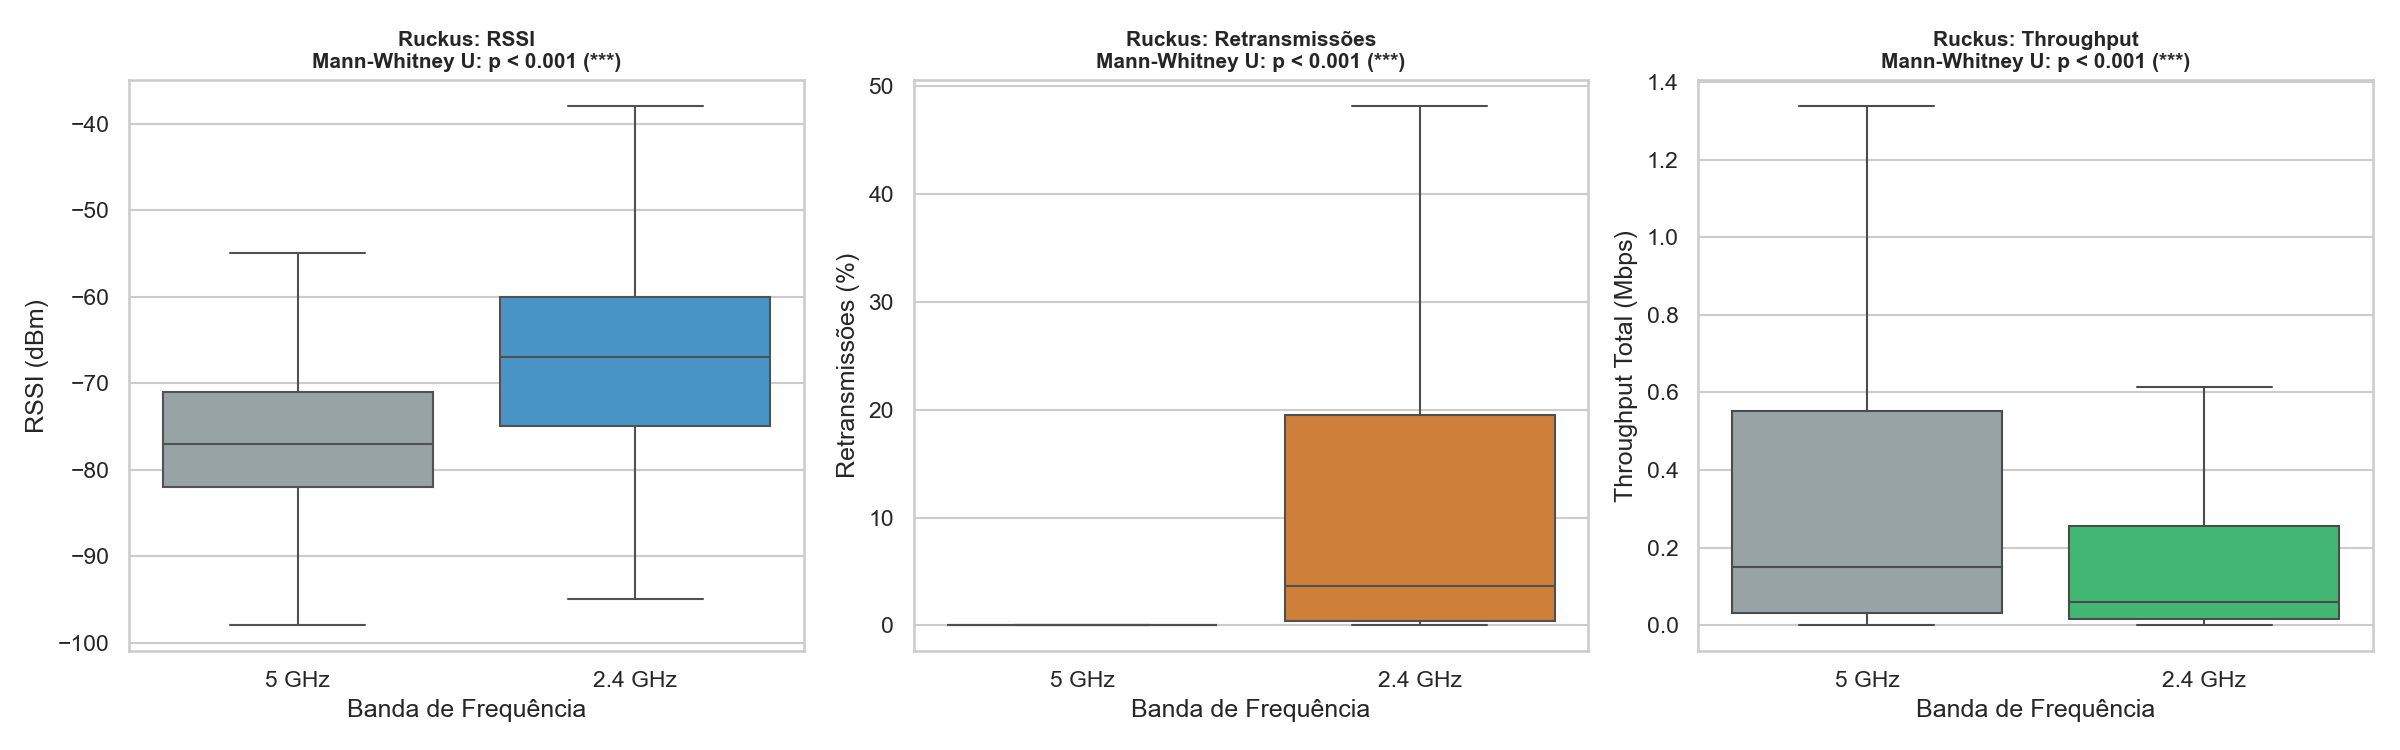
\includegraphics[width=0.85\textwidth]{img/01_ruckus_bandas_comparacao.png}
  \caption{Comparação de Bandas Ruckus}
  \label{fig:01_ruckus_bandas_comparacao_png}
\end{figure}
\begin{itemize}
  \item \textbf{RSSI}: A diferença é altamente significativa ($p < 0,001$) com tamanho de efeito médio (\textit{r} = 0,3619). A mediana em 2,4 GHz é de \texttt{-67.0 dBm} contra \texttt{-77.0 dBm} em 5 GHz, refletindo a física de atenuação do sinal de 5 GHz.
  \item \textbf{Retransmissões}: Diferença estatisticamente significativa ($p < 0,001$) com tamanho de efeito grande (\textit{r} = 0,5221). O 2,4 GHz possui retransmissões médias de \texttt{15.71\%} contra \texttt{1.98\%} do 5 GHz, condizente com a poluição de espectro na frequência mais baixa.
  \item \textbf{Throughput}: Diferença estatisticamente significativa ($p < 0,001$) com tamanho de efeito pequeno (\textit{r} = 0,1634). O throughput médio em 5 GHz (\texttt{0.545 Mbps}) mostra-se superior ao de 2,4 GHz (\texttt{0.257 Mbps}).

  \item \textbf{UniFi}: Omitido devido à indisponibilidade de conexões em 5 GHz na telemetria da UniFi.


\end{itemize}
\subsubsection{Comparação de Fabricantes (Ruckus vs UniFi)}

\paragraph{Geral}
\begin{itemize}
  \item \textbf{Visualização}:
\end{itemize}
\begin{figure}[H]
  \centering
  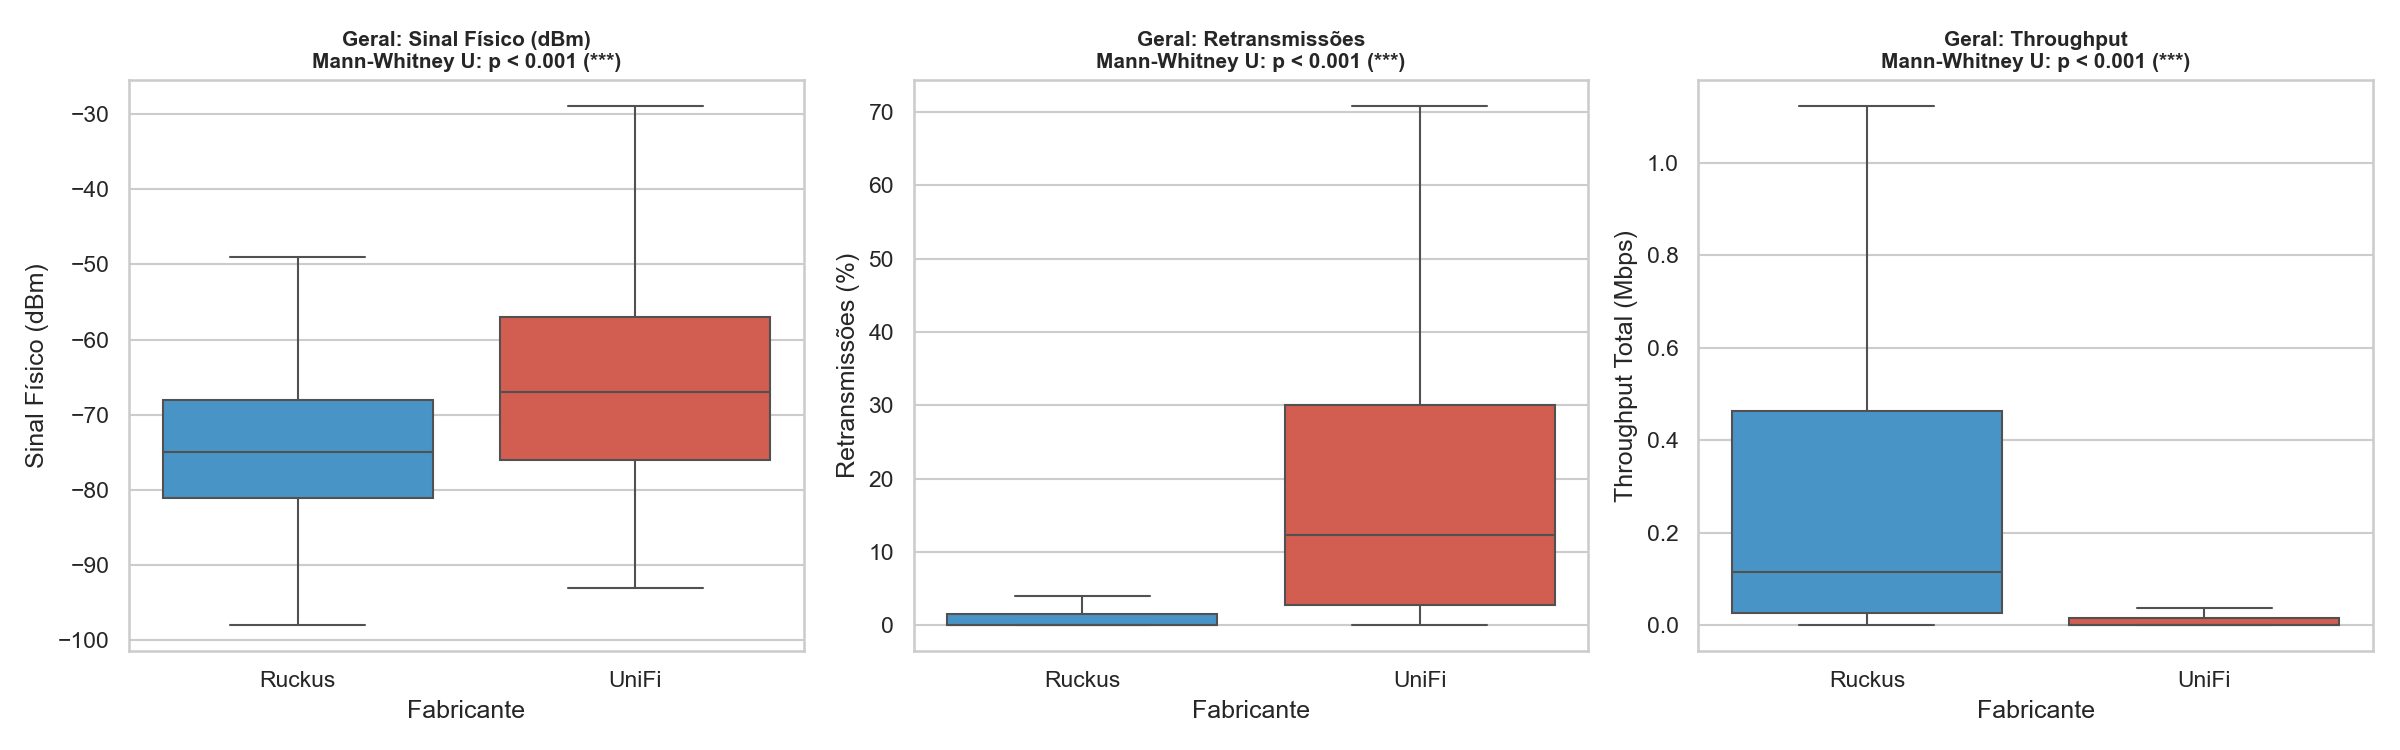
\includegraphics[width=0.85\textwidth]{img/03_fabricantes_geral_comparacao.png}
  \caption{Comparação de Fabricantes Geral}
  \label{fig:03_fabricantes_geral_comparacao_png}
\end{figure}
\begin{itemize}
  \item \textbf{Sinal Físico (dBm)}: A UniFi registrou mediana de sinal físico de \texttt{-67.0 dBm} enquanto a Ruckus registrou \texttt{-75.0 dBm}, diferença significativa ($p < 0,001$) com tamanho de efeito pequeno (\textit{r} = 0,1870). Isso reflete as características físicas específicas dos locais monitorados (escritórios e laboratórios com menor distância média aos APs na UniFi), embora a intensidade do sinal dependa também das antenas, potência de transmissão e características de hardware dos dispositivos clientes.
  \item \textbf{Retransmissões}: A diferença é altamente significativa ($p < 0,001$) com tamanho de efeito médio (\textit{r} = 0,3613). A UniFi apresenta média de \texttt{21.65\%} contra \texttt{5.62\%} do Ruckus. Esta disparidade indica a influência da metodologia de medição: a UniFi estima a retransmissão indiretamente com base no CCQ do firmware, enquanto a Ruckus monitora estritamente a taxa de quadros físicos retransmitidos no rádio.
  \item \textbf{Throughput}: A Ruckus registrou throughput médio de \texttt{0.469 Mbps} contra \texttt{0.257 Mbps} da UniFi, com diferença estatisticamente significativa ($p < 0,001$) e tamanho de efeito médio (\textit{r} = 0,3332). Os resultados sugerem que a rede Ruckus escoou uma taxa superior de dados por cliente no cenário coletado.
  \item \textbf{Índice de Equidade (Jain)}: A comparação da equidade de compartilhamento de throughput entre os clientes conectados simultaneamente revelou diferença estatisticamente significativa ($p < 0,001$) com tamanho de efeito médio (\textit{r} = 0,4484). A Ruckus registrou equidade média de \texttt{0.3427} e mediana de \texttt{0.2637}, enquanto a UniFi obteve média de \texttt{0.1904} e mediana de \texttt{0.1378}. Isso sugere tendências distintas no balanceamento de carga entre os clientes ativos de cada fabricante.

\end{itemize}
\paragraph{Comparações por Banda de 2,4 GHz (Isolado)}
\begin{itemize}
  \item \textbf{Visualização 2,4 GHz}:
\end{itemize}
\begin{figure}[H]
  \centering
  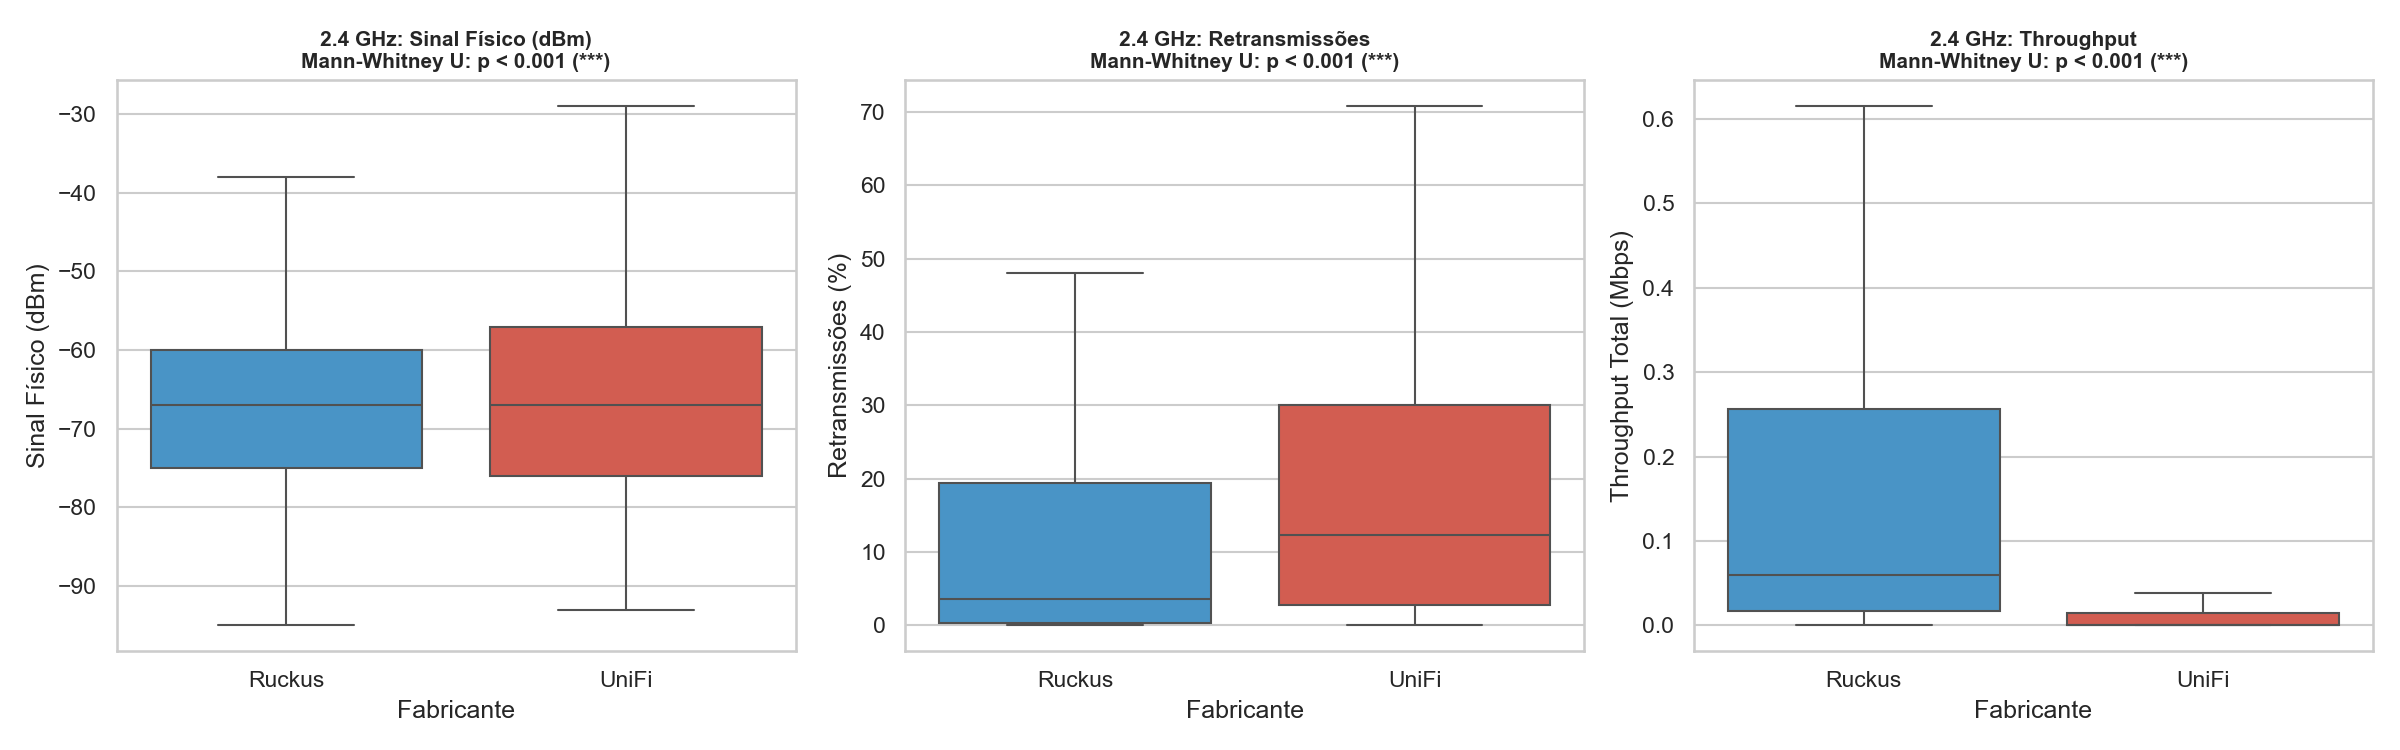
\includegraphics[width=0.85\textwidth]{img/04_fabricantes_24ghz_comparacao.png}
  \caption{Comparação de Fabricantes 2.4 GHz}
  \label{fig:04_fabricantes_24ghz_comparacao_png}
\end{figure}
\begin{itemize}
  \item As tendências observadas no cenário geral se mantêm na frequência isolada de 2,4 GHz: o sinal recebido na UniFi apresenta-se melhor ($p < 0,001$), o throughput médio na Ruckus é superior ($p < 0,001$) e a taxa de retransmissões baseada no CCQ na UniFi mostra-se consideravelmente maior ($p < 0,001$).

\end{itemize}
\paragraph{Comparações por Banda de 5 GHz (Isolado)}
\begin{itemize}
  \item \textit{Nota}: Não é possível realizar a comparação em 5 GHz entre fabricantes, pois a UniFi não registrou telemetria nessa frequência.


\end{itemize}
\subsection{Tabela Detalhada dos Testes de Hipótese}

A tabela abaixo apresenta os mesmos testes estatísticos em formato expandido, contendo os resultados individuais de verificação de normalidade (Shapiro-Wilk), o tipo de teste selecionado (U de Mann-Whitney ou Teste t) e o valor bruto calculado da estatística de teste.

\begin{table}[H]
\IBGEtab{%
  \caption{Tabela Detalhada dos Testes de Hipótese}%
  \label{tab:data_testes_hipotese_2}%
}{%
  \centering\footnotesize
  \resizebox{\textwidth}{!}{%
    \begin{tabular}{lcccccccccc}
      Métrica & Grupo A & Grupo B & Média/Mediana A & Média/Mediana B & Normal A/B & Teste Aplicado & Estatística & P-valor & Tam. Efeito (r / d) & Diferença Significativa? \\
      \midrule
      \textbf{RSSI} & Ruckus 2,4G & Ruckus 5G & -67,304 / -67,000 & -75,984 / -77,000 & Não/Não & Mann-Whitney U & 22691746053,50 & $p < 0,001$ (\textsuperscript{***}) & 0,3619 & \textbf{Sim} \\
      \textbf{Retransmissões} & Ruckus 2,4G & Ruckus 5G & 15,706 / 3,641 & 1,983 / 0,000 & Não/Não & Mann-Whitney U & 32613638143,50 & $p < 0,001$ (\textsuperscript{***}) & 0,5221 & \textbf{Sim} \\
      \textbf{Throughput} & Ruckus 2,4G & Ruckus 5G & 0,257 / 0,060 & 0,545 / 0,150 & Não/Não & Mann-Whitney U & 15236405525,50 & $p < 0,001$ (\textsuperscript{***}) & 0,1634 & \textbf{Sim} \\
      \textbf{RSSI} & UniFi 2,4G & UniFi 5G & 29,576 / 29,000 & N/A & N/A/N/A & Nenhum (Dados Insuficientes) & N/A & N/A & N/A & \textbf{Dados Insuficientes} \\
      \textbf{Retransmissões} & UniFi 2,4G & UniFi 5G & 21,654 / 12,300 & N/A & N/A/N/A & Nenhum (Dados Insuficientes) & N/A & N/A & N/A & \textbf{Dados Insuficientes} \\
      \textbf{Throughput} & UniFi 2,4G & UniFi 5G & 0,257 / 0,000 & N/A & N/A/N/A & Nenhum (Dados Insuficientes) & N/A & N/A & N/A & \textbf{Dados Insuficientes} \\
      \textbf{Sinal Físico (dBm)} & Ruckus & UniFi & -73,753 / -75,000 & -66,223 / -67,000 & Não/Não & Mann-Whitney U & 6889907166,50 & $p < 0,001$ (\textsuperscript{***}) & 0,1870 & \textbf{Sim} \\
      \textbf{Retransmissões} & Ruckus & UniFi & 5,620 / 0,000 & 21,654 / 12,300 & Não/Não & Mann-Whitney U & 3682452798,00 & $p < 0,001$ (\textsuperscript{***}) & 0,3613 & \textbf{Sim} \\
      \textbf{Throughput} & Ruckus & UniFi & 0,469 / 0,116 & 0,257 / 0,000 & Não/Não & Mann-Whitney U & 18886445094,50 & $p < 0,001$ (\textsuperscript{***}) & 0,3332 & \textbf{Sim} \\
      \textbf{Índice de Equidade (Jain)} & Ruckus & UniFi & 0,343 / 0,264 & 0,190 / 0,138 & Não/Não & Mann-Whitney U & 13393982,00 & $p < 0,001$ (\textsuperscript{***}) & 0,4484 & \textbf{Sim} \\
      \textbf{Sinal Físico (dBm)} & Ruckus 2,4G & UniFi 2,4G & -67,304 / -67,000 & -66,223 / -67,000 & Não/Não & Mann-Whitney U & 2579762545,50 & $p < 0,001$ (\textsuperscript{***}) & 0,0300 & \textbf{Sim} \\
      \textbf{Retransmissões} & Ruckus 2,4G & UniFi 2,4G & 15,706 / 3,641 & 21,654 / 12,300 & Não/Não & Mann-Whitney U & 2263260611,50 & $p < 0,001$ (\textsuperscript{***}) & 0,2101 & \textbf{Sim} \\
      \textbf{Throughput} & Ruckus 2,4G & UniFi 2,4G & 0,257 / 0,060 & 0,257 / 0,000 & Não/Não & Mann-Whitney U & 4782877481,00 & $p < 0,001$ (\textsuperscript{***}) & 0,4441 & \textbf{Sim} \\
      \textbf{Sinal Físico (dBm)} & Ruckus 5G & UniFi 5G & -75,984 / -77,000 & N/A & N/A/N/A & Nenhum (Dados Insuficientes) & N/A & N/A & N/A & \textbf{Dados Insuficientes} \\
      \textbf{Retransmissões} & Ruckus 5G & UniFi 5G & 1,983 / 0,000 & N/A & N/A/N/A & Nenhum (Dados Insuficientes) & N/A & N/A & N/A & \textbf{Dados Insuficientes} \\
      \textbf{Throughput} & Ruckus 5G & UniFi 5G & 0,545 / 0,150 & N/A & N/A/N/A & Nenhum (Dados Insuficientes) & N/A & N/A & N/A & \textbf{Dados Insuficientes} \\
      \bottomrule
    \end{tabular}%
  }%
}{%
  \fonte{Produzido pelos autores.}%
}
\end{table}

